\subsection{Structure de l'oeil}

Ce cours \'etudie donc la bouce de traitement des images qui part de l'\'ecran, est analys\'ee par l'oeil et le cerveau et g\'en\`ere des actions qui sont per\c{c}ues par l'ordinateur. Nous nous concentrons ici sur la \textbf{perception visuelle}.

Le point essentiel de ce cours est de montrer \textbf{qu'une grande partie de la perception visuelle se passe dans le cerveau}. C'est le cas de la construction des couleurs, comme nous le verrons plus loin, mais aussi de certaines illussions visuelles, comme la perception du triangle de Nakizsa: les bords du triangle ne sont pas dans l'image mais construits par le cerveau.

\begin{figure}[H]
\centering
\makebox[\textwidth][c]{
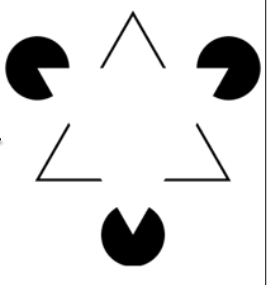
\includegraphics[scale=0.55]{./images/triangle.png}
}
\caption{Triangle de Nakizsa}
\end{figure}

Voici la structure d'un oeil dont 4 \'el\'ements sont particuli\`erement pertinents pour le cours Visual Computing.

\begin{figure}[H]
\centering
\makebox[\textwidth][c]{
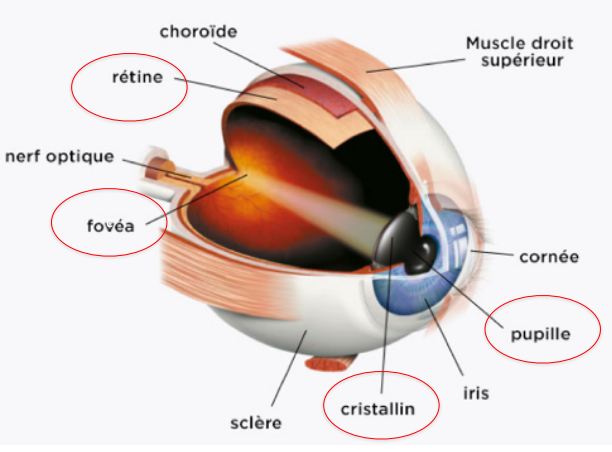
\includegraphics[scale=0.55]{./images/oeil.png}
}
\end{figure}

\begin{itemize}
\item \textbf{pupille}: contr\^ole la quantit\'e de lumi\`ere qui entre dans l'oeil. Sa taille est contr\^ol\'ee par des mouvements des muscles de l'iris qui agissent par r\'eflexe \`a la quantit\'e de lumi\`ere. 
\item \textbf{cristallin}: c'est une lentille bi-convexe qui concentre plus ou moins les rayons lumineux sur la r\'etine. il permet de garder une image nette \`a des profondeurs de champs diff\'erents. Les muscles autour du cristallin l'\'etirent lorsque l'objet regard\'e s'\'eloigne, un ph\'enomene appel\'e \textbf{accomodation}.
\item \textbf{r\'etine}: sorte d'\'ecran plac\'e au fond de l'oeil. Elle est la partie de l'oeil qui capte les photons gr\^ace a un grand nombre de photorecepteurs. Elle couvre le 75 \% de la surface interne de l'oeil.
\item \textbf{macula et fov\'ea}: la macula est la partie centrale de la r\'etine situ\'ee dans l'axe de la r\'etine.  La fov\'ea est une partie de la macula, une p\'etite d\'epression qui correspond \`a la zone qui nous donne la plus grande activit\'e visuelle. Elle comprend une tr\`es forte densit\'e de certains photor\'ecepteurs appel\'ees \textbf{c\^ones} alors que le reste de la macula comporte d'avantage des r\'ecepteurs appel\'es \textbf{b\^atonnets}.
\end{itemize}

Les b\^atonnets et les c\^ones sont des cellules photosensibles. Les b\^atonnets ne per\c{c}oivent pas les couleurs mais sont plus sensibles aux \textbf{niveaux de gris}. Ils permettent notamment la vision par faible luminosit\'e. Ils semblent aussi impliqu\'es dans la \textbf{vision p\'eriph\'erique} pour la perception du mouvement. Environ la r\'etine contient 100 millions.

Les c\^ones se situent dans la fov\'ea. Ils sont environ 6 millions. Ils ont besoin d'avantage de lumi\`ere et sont responsables de la perception de la couleur. En r\'ealit\'e, les c\^ones ne reconnaissent pas la couleur mais nous poss\'edons 3 types de c\^ones sensibles \`a des longueurs d'onde diff\`erentes. Les c\^ones n'envoient pas un message de couleur au cerveau mais lui communiquent le nombre des photons quie les ont heurt\'es. Le \textbf{daltonisme} r\'esulte du fait que certains types de c\^ones ne poss\`edent pas les pigments photosensibles qui captent les photons.

Il existe cependant, dans chaque oeil, une zone d\'epourvue de r\'ecepteurs car c'est le point d'ancrage du nerf optique qui conduit les informations au cerveau. Il s'appelle le \textbf{point aveugle}: tout objet situ\'e dans l'axe r\'etine-point aveugle sera invisible pour cet oeil. Si nous avos les deux yeux ouvert, l'objet sera toujours visible par un oeil. 

En classe, nous font l'exper\'erience suivante. Fermez l'oeil droit. Regardez le losange rouge avec l'oeil gauche. Le professeur traverse l'\'ecran doucement. Vous percevez le professeur en vision p\'eriph\`erique mais il va dispara\^itre un moment.

La structure de la r\'etine d\'efinit notre acurit\'e visuelle dans les diff\'erent zones de notre champ de vision. Notre vision la plus pr\'ecise se limite \`a un angle de 5 degr\'es. N\'eanmoins notre oeil est sensible aux mouvements p\'eriph\'eriques. Il ne glisse pas de mani\`ere continue sur le texte mais l'explore par saccades (voir eye tracking). L'oeil se pose pendant des courtes pauses ou \textbf{fixations} d'un quart de second. Puis, il se d\'eplace tr\`es rapidement vers un autre endroit, ce qu'on appelle une \textbf{saccade}. L'oeil pr\'el\`eve de l'information quand il fait une fixation alors qu'il est aveugle pendant la saccade.

\begin{figure}[H]
\centering
\makebox[\textwidth][c]{
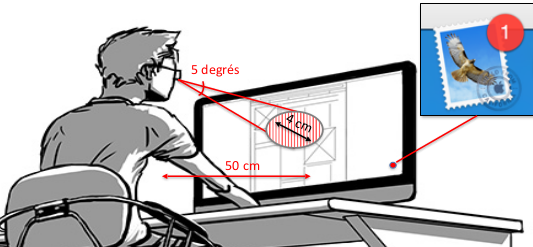
\includegraphics[scale=0.55]{./images/fixation.png}
}
\end{figure}

Quelle quantit\'e d'information visuelle est-elle comprise dans cette zone fov\'eale de 4 cm de diam\`etre?. Cela d\'epend de 6 param\`etres \'enum\`er\'es \`a continuation:

\begin{itemize}
\item l'acurit\'e visuelle de l'utilisateur, de sa distance,de ses lunettes !
\item zoom choisi par l'utilisateur ! 
\item Propri\'et\'es de l'\'ecran:
\begin{itemize}
\item dimensions: longueur de la diagonale (par exemple 13 pouces).
\item d\'efinition: nombre de pixels.
\item r\'esolution: nombre de pixels par pouce carré.
\item profondeur: nombre de bits utilis\'e par chaque pixel.
\end{itemize}

Le	nombre	de	pixels	par	\'ecran	n'a	pas	cess\'e	d’augmenter....
\end{itemize}

Les 3 types de c\^ones envoient chacun un nombre de stimulations \'electriques en fonction du nombre de photons qui les ont heurt\'e. C'est donc le cerveau humain, notamment le \textbf{cortex visuel}, qui int\`egre ces 3 informations pour d\'eterminer la couleur. 

Il semblerait que notre cerveau soit capable de distinguer 10 millions de couleurs. attention, il ne s'agit pas de leur donner un nom mais de d\'etecter que deux couleurs sont diff\'erents. Le nombre de 10 millions d\'epend donc du protocole exp\'erimental utilis\'e, ce qui explique qu'il n'y ait pas consensus. Mais cela signifierait qu'un \'ecran qui a une profondeur de pixel de 24 bits peut g\'en\`erer d'avantage des couleurs que ce que l'oeil humain peut discriminer. 

Dans quelques images on peut voir que la m\^eme diff\'erence en pourcentage de cyande est ou non est perceptible. Il s'explique par la faible pr\'ecision du syst\`eme.

La taille d'un fichier image d\'epend donc du nombre des points dans cette image ainsi que du nombre des bits d'information par point, c'est à dire la profondeur du pixel. Heuresement, ce nombre est ensuite diminu\'e par des \textbf{m\'ethodes de compr\'ession d'image}. D'autres cours de l'EPFL traitent abondamment des m\'ethodes de compression. Apr\'es une compression \textbf{"lossless"}, la d\'ecompression du fichier permet de retrouver exactement chaque bit d'information du fichier original. C'est le cas de fichiers .ZIP. Dans une m\'ethode \textbf{"lossy"}, ce n'est pas le cas. Par example, si on prend la moyenne de couleur entre pixels voisins, un pixel blanc et un noir deviendront deux pixels gris apr\'es la d\'ecompression on pourra d\'eterminer s'ils s'agissait au d\'epart de deux gris ou d'un blanc et d'un noir. La question est de savoir combien d'information peut \^etre perdu \`a la d\'ecompression sans que l'oeil humain ne s'en aper\c{c}oive. En ce qui concerne les images, les standards \textbf{PNG} et \textbf{GIF} sont "lossless" alors que \textbf{JPEG} est "lossy".

\subsection{L'effet Stroop}

Les transparents qui pr\'ec\`edent concernaient la capacit\'e de distinguer deux couleurs. Il ne s'agisait pas de les nommer, ce qui est une t\^ache cognitive (retrouver le nom dans sa m\'emoire \`a long-terme). Voici une exp\'erience qui montre les interf\'erences entre la perception et la cognition. 

\begin{figure}[H]
\centering
\makebox[\textwidth][c]{

\includegraphics[scale=0.55]{./images/stroop.png}
}
\end{figure}

Stroop a d\'ecouvert un effet int\'eressant li\'e \`a la t\^ache suivante: le sujet doit lire un nom de couleur \'ecrit soit dans la couleur du nom soit dans une autre couleur. Il faut nommer la couleur du mot. L'experience au CHILI est un peu diff\'erente: il faut dire si l'\'enonc\'e est correct. 

Le temps n\'ecessaire pour \'enoncer la couleur d'un mot est plus \'elev\`ee si le mot d\'esigne une autre couleur. Ce ph\'enomene \textbf{d'interf\'erence} r\'esulte du fait qu'on ne puisse s'emp\^echer de lire le mot, de lui donner une \textbf{valeur s\'emantique}. La perception ne se fait de mani\`ere independante des autres activit\'es du cerveau, comme nous allons continuer \`a le d\'emontrer.

Comme illustr\'e au d\'ebut de ce cours, la couleur n'est pas per\c{c}ue par l'oeil mais reconstruite par le cortex visuel en fonction du nombre de signaux re\c{c}us par les trois types de c\^ones. C'est aussi dans le cerveau que se construisent la perception du mouvement, les effets d'amor\c{c}age et la perception de la profondeur.

\subsection{Perception du mouvement}

La perception du mouvement doit forc\'ement r\'esulter de la sucession d'images, celles-ci ne sont pas gard\'ees dans l'oeil mais envoy\'ees instantann\'ement au cerveau. Les avis divergent sur le nombre d'images qu'un oeil peut percevoir par secondes. Il semblerait que la r\'etine puisse capter plus de 100 images par seconde (entre 75 et 150), certains parlent de 1000 fps, le point est controvers\'e. Alors pourquoi le cin\'ema s'est-il fix\'e sur le standard de 24 images par secondes? Parce qu'avec 24 images par secondes, voire \`a partir de 16, nous percevons les mouvements commme \'etant continus. Ce nombre de 24 ne r\'epose pas sur une r\'ealit\'e physiologique mais sur un standard \'etablit aux premi\'eres heures du cin\`ema. Aujourd'hui certaines TV haut r\'esolution proposent 120 images par secondes voire 240 pour les \'ecrans LEDs, on parle m\^eme de TV \`a 480 fps. Le d\'ebat consiste \`a savoir si ces fr\'equences offrent une diff\'erence perceptible de confort visuel.

Pourquoi per\c{c}oit-on des images qui se suivent comme un mouvement continu?

\subsubsection{Hypoth\`ese 1: persistence r\'etinienne}

La premi\`ere hypoth\`ese, aujourd'hui critiqu\'ee par les scientifiques, mais toujours r\'epandue dans l'opinion publique, serait que la r\'etine garde un moment l'information avant que les cellules photor\'eceptrices qui ont \'et\'e excit\'ees par un photon ne retournent \`a leur \'etat de repos.

L'image resterait environ entre 1/12 et 1/25 de seconde "imprim\'ee" dans la r\'etine, donc, d\`es 24 images par seconde, on percevrait une continuit\'e. Le film du cheval ne comporte que 12 images par seconde, on voit que le mouvement n'est pas fluide mais on re\c{c}oit n\'eanmoins le mouvement. L'hypoth\`ese de la persistence r\'etinienne est aujourd'hui abandonn\'ee au profit de l'hypoth\`ese suivante.

\subsubsection{Hypoth\`ese 2: effet phi et effet beta}

L'effet phi est la sensation visuelle de mouvement provoqu\`ee par l'apparition d'images per\c{c}ues successives, susceptibles d'\^etres raccord\`ees par un d\'eplacement ou une transformation. C'est le cerveau qui "comblerait" les images interm\'ediaires, qui imagine le mouvement. L'effet beta est la m\^eme illusion de mouvement cr\'e\'e par des images statiques, alors que l'effet phi repose sur des images qui clignotent.

En r\'esum\'e, les hypoth\`eses qui attribuent la construction de la continuit\'e du mouvement au cerveau dominent aujourd'hui celles qui l'attribuent \`a l'oeil. Ce ph\`enom\`ene qui expliquerait le mouvement apparent dans les "flipbooks" et "thaumatropes".

\subsection{Perception de l'amor\c{c}age}

La perception est typiquement en m\'ecanisme bottom-up: je per\c{c}ois l'image d'un objet et je l'associe aux objets que je connais d\'ej\`a. On parle de processus-bottom up: l'image de l'objet s'imprime sur la r\'etine qui transmet au cortex visuel lequel communique avec les autres composantes du syst\`eme cognitif.

Ce texte illustre le processus \textbf{bottom-up}:

Le fait qu'un \'el\'ement visuel brise la r\'egularit\'e du texte. Rome \'etant \'ecrit en rouge, permet de le s\'electionner plus rapidement. 
Le fait que Rotterdam se mette \`a trembler attire notre attention.
Le fait que Moscu se d\`epala attire notre attention.

Parmi l'ensemble des stimuli pr\'esent\'es, certains ont des propri\'et\'es qui attirent notre attention, celui-ci brise une r\`egularit\`e \'etablie par l'ensemble du stimulus.

\begin{figure}[H]
\centering
\makebox[\textwidth][c]{

\includegraphics[scale=0.35]{./images/cites.png}
}
\end{figure}

Dans cette image, le taxi en couleur \'eclatante d\'eclenche les processus bottom-up. Notre attention devrait donc surtout s\'electionner le taxi. Mais un autre processus intervient: il n'est pas normal de voir un \'el\'ephant en libert\'e dans les rues d'une ville. Sa pr\'esence entre en conflit avec ce qu'on attend en regardant une image de ville nocturne...Dans ce cas, c'est notre cognition qui dirige notre attention et non pas les propri\'et\'es physiques de l'image qui guident l'attention. On parle dans ce cas de processus \textbf{top-down}. La perception d'objets dans une image est fortement influenc\'ee par nos attentes, nos exp\'eriences, nos connaissances,...La perception d'objets dans une image est fortement influenc\'ee par nos attentes, nos exp\'eriences, nos connaissances,...

\begin{figure}[H]
\centering
\makebox[\textwidth][c]{
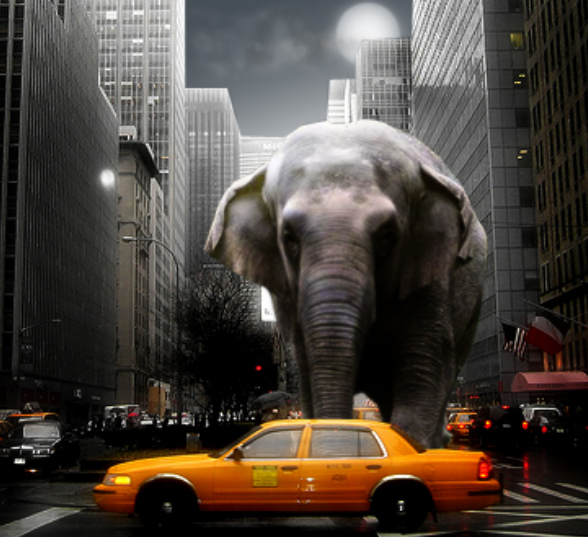
\includegraphics[scale=0.35]{./images/elephant.png}
}
\end{figure}
	
\textbf{L'effet d'amor\c{c}age ou priming effect} consiste \`a pr\'esenter un stimulus (l'amorce) afin d'influencer la perception d'un autre stimules (la cible). L'amorce \'etait les images pr\'ealables de vase ou de profils et la cible \'etait l'image ambigue. Nous percevons beacoup d'objets mais les processus bottom-up guident notre attention sur certains objets particuliers, c'est \textbf{l'attention s\'elective}. Un example bien connu dans la perception auditive est le \textbf{cocktail party effect}: si je parle avec plusieurs personnes au milieu d'une soir\'ee bruyante, je per\c{c}ois n\'eanmoins les conversations externes car, si quelqu'un prononce mon nom une autre table, ceci attirera n\'eanmoins mon attention.

\begin{figure}[H]
\centering
\makebox[\textwidth][c]{
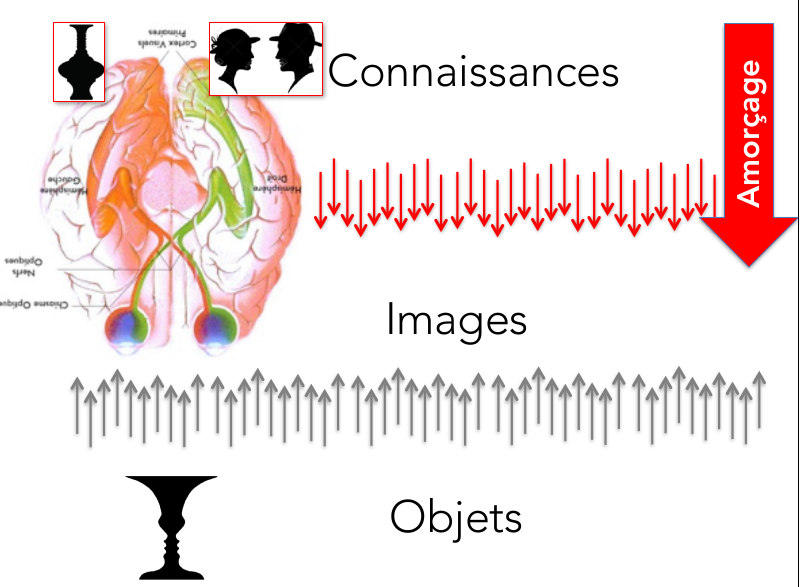
\includegraphics[scale=0.35]{./images/amorce.png}
}
\end{figure}

\subsection{Perception de la profondeur}

La perception de la profondeur est construite par le cerveau qui r\'econcilie les informations provenant des deux yeux. Chaque oeil envoie un demi-champ de vision \`a chaque h\'emisph\`ere. Il utilise des indices diff\'erents:

\subsubsection{Indices binoculaires}

Le principe de base est simple, l'angle de l'image sur la r\'etine d\'etermine la distance d l'objet par triangulation.

\subsubsection{Indices monoculaires}

M\^eme avec un seul oeil ouvert, nous avons une certaine perception de la profondeur gr\^ace \`a diff\'erents indices. 

\textbf{La perspective}: deux lignes parall\`eles qui s'\'eloginent du point de vision sont per\c{c}ues comme se rapprochant. On peut en profiter avec un oeil ferm\'e mais il n\'ecessite un d\'eplacement ce qui n'est pas tr\'es diff\'erent d'un principe binoculaire ou multioculaire.

\textbf{L'effet parralaxe}: c'est un m\'ethode pour obtenir la profondeur en faisant d\'eplacer les objets en premier plan plus rapidement que les objets en deuxi\`eme plan.

\textbf{L'effet kinetic depth}: les mouvements de l'objet donnent une perception de sa structure en 3D.


\begin{figure}[H]
\centering
\makebox[\textwidth][c]{
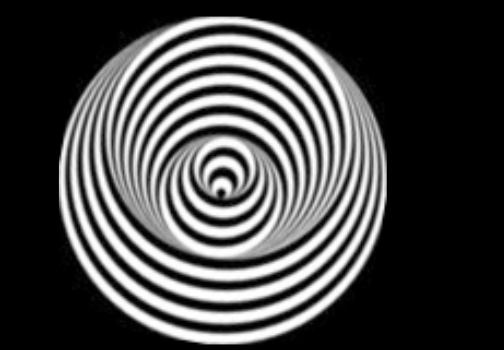
\includegraphics[scale=0.35]{./images/kinetic.png}
}
\end{figure}

\textbf{L'occlussion}: m\^eme en 2D, cette image donne l'impression que le rectangle jaune se trouve en avant-plan du rectangle bleu. Cet effet peut \^etre retourn\'e, par exemple si la forme bleu n'est pas un rectangle mais un polygone en forme de U couch\'e. Les ombres constintuent un cas particulier d'occlusion.

\begin{figure}[H]
\centering
\makebox[\textwidth][c]{
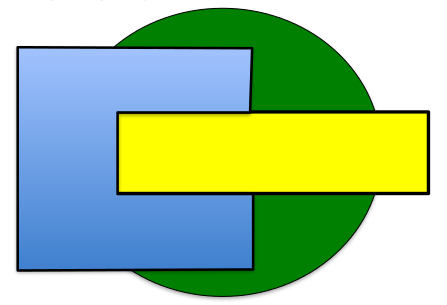
\includegraphics[scale=0.35]{./images/occlusion.png}
}
\end{figure}

\textbf{La taille relative}:

Malgr\'e l'absence de lignes de perspective, les objets plus petits sont per\c{c}us comme plus \'elogin\'es, sauf si la s\'emantique de l'image nous fournit une autre interpr\'etation de la diff\'erence de taille. Sans indices externes, on ne peut estimer la distance d'un objet dont on ne conna\^it pas la taille. 

\textbf{Position par rapport \`a l'horizon}:

Le fait de briser la ligne d'horizon est une propri\'et\'e des objets \'eloign\'es.

\subsection{Recr\'eer la profondeur en 2D}

La diff\'erence de nettet\'e de l'image entre l'avant plan et l'arri\`ere plan fournit une perception de la profondeur. 

\textbf{Finesse de la texture}: la profondeur est communiqu\'ee en augmentant la finesse des textures en avant plan et en la r\'eduisant dans le fond.

\textbf{Brouillard de distance}: un effet brouillard est utilis\'ee dans les jeux pour donner une perception de la profondeur. Il permet aussi de ne pas calculer les d\'ecors tr\`es \'eloign\'es.

\subsection{Remarques}

Chaque h\'emisph\`ere traite une demi-image et la partage avec l'autre h\'emisph\`ere. Mais que se passe-t-il si l'information ne passe plus entre les deux h\'emisph\`eres? Ceci arrive notamment dans des cas graves d'\'epilepsie qui conduit \`a une intervention chirugical qui sectionne le corps calleux, le faisceau d'axones qui connecte les deux h\'emisph\`eres.

\begin{figure}[H]
\centering
\makebox[\textwidth][c]{
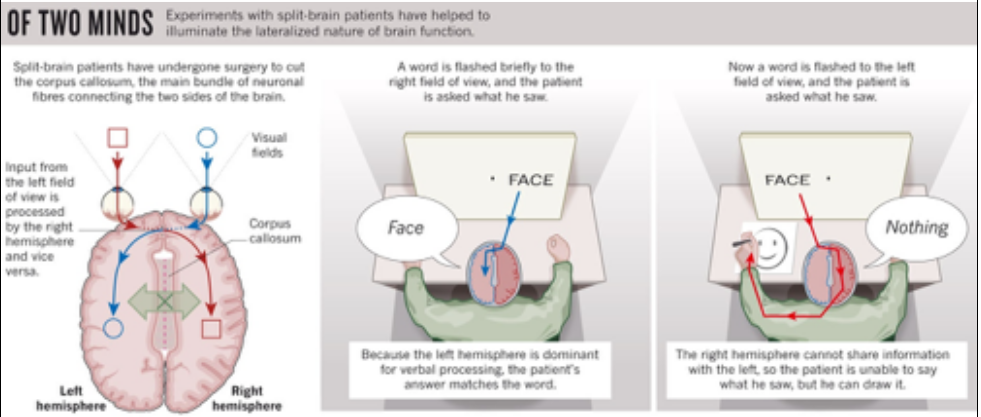
\includegraphics[scale=0.35]{./images/splitbrain.png}
}
\end{figure}

\textbf{Exp\'erience du Split Brain}: gr\^ace \`a un dispositif technique, on projectte par exemple deux demi-images droites qui ne sont envoy\'ees qu'\`a l'hemisph\`ere gauche. Celui-ci \'etant sp\'ecialis\'e dans le traitement du langage, le sujet peut dire "face". Si ces deux demi-images sont transmises \`a l'h\'emisph\`ere droit, le sujet ne pourra pas lire le mot mais pourra dessiner l'objet.

\textbf{Stimuli subliminaux} (hypoth\`ese controvers\'ee):
\begin{itemize}
\item Si un stimulus visuel est inf\'erieur au seuil de perception (en taille, dur\'ee, longueur d'ondes), il serait n\'eanmoins per\c{c}u par notre inconscient.
\item Il aurait de ce fait une influence non-contr\^olable sur notre comportement.
\end{itemize}

\subsection{Exercises}

\begin{exercise}
Quelles composantes de l'oeil lui permettent de r\'ealiser les performances suivantes?
\end{exercise}
\begin{itemize}
\item Lire des petits caract\'eres \`a l'\'ecran. (cristallin)
\item Discriminer un mot en bleu d'un mot en rouge. (c\^ones)
\item S'adapter \`a la distance de l\'ecran pour obtenir une image nette. (cristallin)
\item Lisant du texte en haut de l'\'ecran, d\'etecter que l'ic\^one mail se met \`a clignoter en bas d'\'ecran (b\^atonnets)
\item Lors d'une promenade nocturne, reconna\^itre des objets dans la p\'enombre (b\^atonnets)
\end{itemize}

\begin{exercise}
O\`u se passent les ph\'enom\`enes suivants? 
\end{exercise}
\begin{itemize}
\item L'effet stroop (cerveau)
\item La persistance de l'image (oeil)
\item L'effet phi ou beta (cerveau)
\item L'effet parallaxe (cerveau)
\end{itemize}











